\documentclass[t, pdftex]{beamer}
\usetheme[]{Cockrell}
%\usetheme[dept=Mechanical\ Engineering]{cockrell}

% \useoutertheme[subsection=false]{miniframes}
% \useoutertheme[footline=authortitle]{miniframes}
% \setbeamercolor{mini frame}{fg=white,bg=utblack}
%\usepackage{etoolbox}
%\patchcmd{\sectionentry}{\usebeamercolor[fg]{section in head/foot}}{\usebeamercolor[fg]{mini frame}}{}{}

\mode<presentation> {	
	% The Beamer class comes with a number of default slide themes	
	% which change the colors and layouts of slides. Below this is a list	
	% of all the themes, uncomment each in turn to see what they look like.
	
		
	%\usetheme{default}	
	%\usetheme{AnnArbor}	
	%\usetheme{Antibes}	
	%\usetheme{Bergen}	
	%\usetheme{Berkeley}	
	%\usetheme{Berlin}	
	%\usetheme{Boadilla}	
	%\usetheme{CambridgeUS}	
	%\usetheme{Copenhagen}	
	%\usetheme{Darmstadt}	
	%\usetheme{Dresden}	
	%\usetheme{Frankfurt}	
	%\usetheme{Goettingen}	
	%\usetheme{Hannover}	
	%\usetheme{Ilmenau}	
	%\usetheme{JuanLesPins}	
	%\usetheme{Luebeck}	
	%\usetheme{Madrid}	
	%\usetheme{Malmoe}	
	%\usetheme{Marburg}	
	%\usetheme{Montpellier}	
	%\usetheme{PaloAlto}	
	%\usetheme{Pittsburgh}	
	%\usetheme{Rochester}	
	%\usetheme{Singapore}	
	%\usetheme{Szeged}	
	%\usetheme{Warsaw}	
	
	% As well as themes, the Beamer class has a number of color themes	
	% for any slide theme. Uncomment each of these in turn to see how it	
	% changes the colors of your current slide theme.
	
	%\usecolortheme{albatross}	
	%\usecolortheme{beaver}	
	%\usecolortheme{beetle}	
	%\usecolortheme{crane}	
	%\usecolortheme{dolphin}	
	\usecolortheme{dove}	
	%\usecolortheme{fly}	
	%\usecolortheme{lily}	
	%\usecolortheme{orchid}	
	%\usecolortheme{rose}	
	%\usecolortheme{seagull}	
	%\usecolortheme{seahorse}	
	%\usecolortheme{whale}	
	%\usecolortheme{wolverine}
	
		
	\setbeamertemplate{footline} % To remove the footer line in all slides uncomment this line	
	%\setbeamertemplate{footline}[page number] % To replace the footer line in all slides with a simple slide count uncomment this line	
	
	%\setbeamertemplate{navigation symbols}{} % To remove the navigation symbols from the bottom of all slides uncomment this line
    
    \setbeamertemplate{itemize item}{\color{utblack}$\blacktriangleright$}
}

% Additional Settings
% From:
% https://tex.stackexchange.com/questions/37127/how-to-remove-some-pages-from-the-navigation-bullets-in-beamer/45038#45038
\makeatletter
\let\beamer@writeslidentry@miniframeson=\beamer@writeslidentry
\def\beamer@writeslidentry@miniframesoff{%
    \expandafter\beamer@ifempty\expandafter{\beamer@framestartpage}{}% does not happen normally
    {%else
        % removed \addtocontents commands
        \clearpage\beamer@notesactions%
    }
}
\newcommand*{\miniframeson}{\let\beamer@writeslidentry=\beamer@writeslidentry@miniframeson}
\newcommand*{\miniframesoff}{\let\beamer@writeslidentry=\beamer@writeslidentry@miniframesoff}
\makeatother

% Additional packages
\usepackage[]{algorithm}
\usepackage{algorithmic}
\usepackage{multicol}
% \usepackage{subfig}
\usepackage[english]{babel}
\usepackage{blindtext}
\usepackage{color}
\usepackage{cancel}
% \usepackage[]{algorithm2e}
\usepackage{mathtools}
\usepackage{amsmath}
\usepackage{pgfgantt}
\usepackage[version=3]{mhchem} % Package for chemical equation typesetting \ce{}
\usepackage{siunitx} % Provides the \SI{}{} and \si{} and \number{}

\renewcommand{\CancelColor}{\color{utorange}}

% Additional Graphics Paths
\graphicspath{{./figs/}{../../../}{./}}

% Custom symbols and operators
\DeclareMathOperator*{\E}{\mathbb{E}}

% Bibliography definition
% \bibliography{../../dissertation/sections/refs.bib}
% \usepackage[style=ieee]{biblatex}
% \bibliography{../../../dissertation/sections/refs.bib}

\title{A CFD-Informed Hi2Low Method for Improving Subchannel Resolution Crud Predictions}
\subtitle{}
\author{William Gurecky}
\date{\today}


\begin{document}
\setbeamertemplate{caption}{\raggedright\insertcaption\par}
\setbeamertemplate{caption}{%
\begin{beamercolorbox}[wd=.5\paperwidth, sep=.2ex]{block body}\insertcaption%
\end{beamercolorbox}%
}

% =========================================================================== %
\titleframe
\frame{\frametitle{Outline}\tableofcontents}

% =========================================================================== %
\section{Introduction}
\subsection*{Crud Background}
\begin{frame}
\frametitle{Chalk River Unidentified Deposit (crud)}
\vspace{-12pt}
Crud forms a porous layer on the surface of fuel rods and is primarily comprised of \ce{NiFe_2O_4} (Nickel Ferrite).
\[
    \frac{d N_{\mathrm{\ce{NiFe}},c}}{dt} = (\alpha_{\mathrm{nb}} + \alpha_{b}q''_{b} )N_{\mathrm{\ce{NiFe}}, \mathrm{cool}} - \gamma_k k
\]
\begin{tiny}
    \begin{itemize}
    \item Where $N_{NiFe,c}$ is the concentration of \ce{NiFe_2O_4} in a small volume on the cladding surface. $N_{NiFe,cool}$ is the concentration of nickel and iron particulates in the coolant.  $k$ is the near-cladding surface turbulent kinetic energy.  $q''$ is the boiling heat flux (only has nonzero value at $T_s>T_{sat}$).  $\alpha_{nb}$ is a non-boiling coefficient and $\alpha_b$ is a boiling rate constant.  $\gamma_k$ is an erosion multiplier.
    \item Preferentially deposited where temperature is high - near or above saturation point - and where local shear stresses on the rod are low.
	\item Crud an increase oxide ingress rates in certain zirc alloys leading to crud induced local corrosion (CILC).
    \item Crud tends to uptake and retain boron from the coolant which drives
          crud induced power shift (CIPS). Also known as axial offset anomaly (AOA).
    \item CASL developed CRUD simulation package, MAMBA, which is integrated with the VERA core simulator providing.  
    \end{itemize}
\end{tiny}
%\begin{figure}[!htbp]
%\centering
%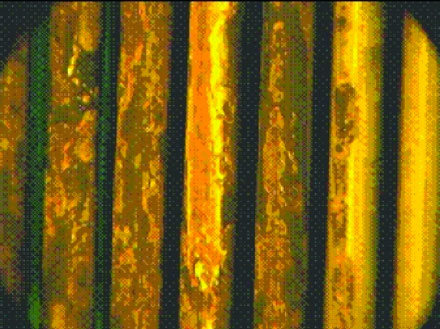
\includegraphics[width=4cm]{figs/crud-crud.jpg}
%\caption{CRUD on fuel rods.}
%\label{log_closed}
%\end{figure}
\vspace{-12pt}
    \begin{figure}
        \centering
        \begin{minipage}{.5\textwidth}
            \centering
            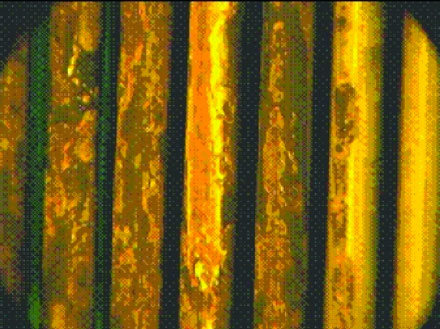
\includegraphics[width=0.55\textwidth]{figs/crud-crud.jpg}
        \end{minipage}%
        \begin{minipage}{.5\textwidth}
            \centering
            \includegraphics[width=0.55\textwidth]{figs/crud_flake_ex.png}
        \end{minipage}
    \end{figure}
\end{frame}

% =========================================================================== %
\subsection*{Motivation}
\begin{frame}
    \frametitle{Crud Induced Power Shift (CIPS)}
    \begin{figure}
        \centering
        \begin{minipage}{.5\textwidth}
            \centering
            \includegraphics[width=6cm]{figs/ao_mpact_ctf.png}
            \caption{Core averaged \% axial offset.  [CASL-I-2015-0318-000]}
        \end{minipage}%
        \begin{minipage}{.5\textwidth}
            \centering
            \includegraphics[width=6cm]{figs/core_b10_mpact_ctf.png}
            \caption{VERA WBNP1 Cycle 7 CRUD \ce{^{10}B}. \\ $@ 16.08 [MWD/MTU]$}
        \end{minipage}
    \end{figure}
\end{frame}

% =========================================================================== %
\subsection*{Motivation}
\begin{frame}
\frametitle{Crud Impacts on Industry}
\vspace{-12pt}
\begin{itemize}
    \item CIPS influences the burnup distribution reducing overall fuel utilization and can reduce shutdown margin  \cite{lange17}.
    \item Plants seeking power uprates or lifetime extensions must prove the facility can operate within thermal limits.  Crud can complicate the analysis by shifting the power distribution and influencing surface heat transfer behavior which must be accounted for in DNB computations.
    \item Though rare, CILC failures require impacted assemblies to drastically reduce power and miss their burnup target.
    \item Crud ultrasonic/chemical shock treatment is an extra step to perform during reloading operations, costing time and potentially increasing radiation exposure risk to plant workers.
\end{itemize}
\textbf{Goal:} Provide predictive capability to avoid CIPS limited fuel loading patterns.
\end{frame}

% =========================================================================== %
\subsection*{Motivation}
\begin{frame}
\frametitle{Current Crud Model Deficiencies}
\begin{itemize}
    \item \textbf{Incorrect boundary conditions provided to the crud code.}
    \begin{itemize}
        \item Fine scale flow details around spacer grids are not resolved by subchannel codes.  It is imperative for CILC analysis to capture the influence of the spacer grids on the crud deposition rate.  
        \item It is also important to account for the presence of spacer grids on crud growth when predicting CIPS.
    \end{itemize}
    \item Incorrect simulated crud chemistry, pore fill mechanisms, and intra-crud species transport models.
    \item Difficulty accounting for the source of corrosion products and nickel and iron particulate entrained in the primary coolant loop.
    \begin{itemize}
        \item Requires understanding of the metallurgy of all primary loop components. 
        \item Plants of different make and vintage require a predictive corrosion and erosion source term models.
    \end{itemize}
\end{itemize}
\end{frame}


% =========================================================================== %
\subsection*{Hi2lo Overview}
\begin{frame}
\frametitle{Hi2lo}
\begin{figure}[]
    \vspace{-16.5pt}
    \centering
    \includegraphics[width=0.99\textwidth]{figs/mamba_hi2lo_vera.png}
    \label{hi2lo_overview}
\end{figure}
\vspace{-16.5pt}
\begin{itemize}
    \item Information flows from high fidelity (CFD) to low fidelity model (CTF) in a unidirectional manner.
    \item Hi2lo augments CTF solution to provide increased fidelity cladding surface temperature, near-wall TKE, and boundary heat flux estimates to MAMBA.
\end{itemize}
\end{frame}


% =========================================================================== %
\subsection*{State of Hi2lo}
\begin{frame}[shrink=10]
\frametitle{Prior Hil2o Work: HTC Remapping Hi2Low Procedure}
\begin{columns}
    \begin{column}{0.5\textwidth}
        \begin{itemize}
            \item Salko et. al (2017)  developed a Hi2Low procedure based on mapping and re-scaling CFD results onto an intermediate reconstruction grid upon which CRUD is grown.
            \item The single phase heat transfer coefficient (HTC) and TKE surface fields are mapped.
            \item An iterative method is used to converge on the correct pin surface temperature given HTC and the boundary heat flux provided by CTF.
        \end{itemize}
    \end{column}
    \begin{column}{0.5\textwidth}  %%<--- here
        \begin{center}
            \begin{figure}
                \includegraphics[width=6cm]{figs/cfd_ctf_multi_grid.png}
                \caption{\centering TKE remapping procedure. \cite{salko17}}      
            \end{figure}
        \end{center}
    \end{column}
\end{columns}
\vspace{-12pt}
\end{frame}

% =========================================================================== %
\subsection*{State of Hi2lo}
\begin{frame}
\frametitle{Prior Hil2o Work: HTC Remapping Hi2Low Procedure}
\begin{figure}[!htbp]
\centering
\begin{minipage}{.5\textwidth}
    %
    \includegraphics[width=5cm]{figs/ctf_crud_orig.png}
    \caption{\centering \scriptsize{ CRUD growth on the rod surface \\ prior to HTC and TKE \\ field remapping.}}
    \label{fig:crud_pre_map}
\end{minipage}%
\begin{minipage}{.5\textwidth}
    %
    \includegraphics[width=5cm]{figs/ctf_crud_reconstructed.png}
    \caption{\centering \scriptsize CRUD growth on the rod \\ surface post HTC and TKE \\ field remapping.}
    \label{fig:crud_post_map}
\end{minipage}
\end{figure}
\end{frame}

% =========================================================================== %
\subsection*{High Fidelity Crud Simulation}
\begin{frame}[shrink=20]
    \frametitle{Coupled CFD/Crud Calculation}
    \begin{itemize}
    \item CFD/Crud coupling is useful for single-pin or single-assembly CRUD estimates.  Fine scale flow near spacer grid impacted surface crud distribution.  Important for quantifying crud induced local corrosion (CILC) risk.
    \item CFD/Crud simulations are too numerically costly for full core simulation.
    \end{itemize}
        \begin{figure}[!htbp]
\centering
\includegraphics[width=0.99\textwidth]{figs/combo_180x.png}
\label{log_closed}
    \end{figure}
\end{frame}

% =========================================================================== %
\subsection*{CFD and Subchannel Mesh Background}
\begin{frame}
Differences between CTF (subchannel) and CFD meshes for a single pin.
\begin{figure}
        \centering
        \begin{minipage}{.4\textwidth}
            \centering
            \includegraphics[width=3cm]{figs/cfd_ctf_mesh_v.png}
        \end{minipage}%
        \begin{minipage}{.4\textwidth}
            \centering
            \includegraphics[width=2cm]{figs/ctf_mesh_v.png}
        \end{minipage}
\end{figure}
\end{frame}

% =========================================================================== %
\section{Approach}
\begin{frame}
    \frametitle{CFD informed surrogate model to improve CRUD growth}
    \begin{itemize}
    \item Construct a scale bridging model which utilizes a suite of precomputed CFD solutions to improve CRUD predictions given on the CTF grid. 
    \item CTF estimates mean TH conditions everywhere in the core at a low spatial resolution.  The surrogate provides higher order moments about the mean.
    \end{itemize}
    \begin{block}{Rod Surface Field}
        \[ 
        F(\mathbf z) = \underbrace{\mu(\mathbf{z})}_\text{CTF} + \underbrace{\varepsilon(\mathbf z, {\mathbf p(\mathbf z)}) + b(\mathbf{z}) }_\text{CFD Informed}
        \]
    \end{block}
    Treat $\varepsilon$ as a random field.  $\varepsilon(\cdot)$ is a CFD informed model. $\mathbf z$ are spatial coordinates. $\mathbf p$ are a set of auxiliary predictors. \\
    $b$ is bias ($\mu_{CTF} - \mu_{CFD}$) \\
    $\mu$ is piecewise constant over each CTF patch
\end{frame}

% =========================================================================== %
\begin{frame}\frametitle{Objectives}
\begin{itemize}
\item Account for fine scale flow features unresolved by CTF on the growth of CRUD and boron hideout.
\item Proposed hi2lo approach:
\begin{itemize}
	\item Forgo attempting to capture spatial distributions of temperature, boundary heat flux and TKE on rod surface. 
	\item Instead, track joint probability density $f(T, TKE, q'')$ tallied over coarse CTF patches.
\end{itemize}
	\item Predict likelihood of temperatures in excess of saturation occurring in coincidence with low local turbulent kinetic energy.
	\item Preserve correlations between surface temperature, boundary heat flux and turbulent kinetic energy.
\end{itemize}
\end{frame}


% =========================================================================== %
\subsection*{Crud State vs Thermal Hydraulic Surface Conditions Covariance Structure}
\begin{frame}
\begin{figure}[]
\vspace{-16.5pt}
\centering
\includegraphics[width=10.88cm]{figs/ctf_patch_ex3_b.png}
\label{model_overview}
\end{figure}
\end{frame}

% =========================================================================== %
\subsection*{CFD vs Subchannel:  Influcene on crud predictive capability}
\begin{frame}
On a single coarse CTF patch:
\vspace{-6.5pt}
\begin{figure}[!htbp]
\centering
\includegraphics[width=11cm]{figs/model_relations_2.png}
\label{model_overview}
\end{figure}
\end{frame}

% =========================================================================== %
\section[Theory]{Theory}
\subsection*{Problem Statement}
\begin{frame}
\textbf{Goal:} Compute the total integrated crud over a CTF patch with area $A$, for a single time step of $\delta t$.
\begin{itemize}
	\item Expected total crud over patch : 
	\begin{eqnarray}
		A \mu_g\ [grams] = A \E[g(\mathbf x|g_o, \mathbf I, \delta t)] \nonumber \\
		= A \iiint g(\mathbf x|g_o, \mathbf I, \delta t) h(\mathbf x|\theta) d \mathbf x  \nonumber
	\end{eqnarray}
	let $\mathbf x= \{T, k, q''\}$.
	$\mathbf I$ represents additional crud parameters, $g_o$ is the crud state at the start of the time step and $\theta$ are distribution parameters.
	\item Estimate this integral via Monte Carlo:
	\[
	\E[g(x)] \approx \frac{1}{N} \sum_i^N \frac{g(\mathbf x_i) 
	h(\mathbf x_i | \theta)}{\tilde h(\mathbf x_i | \tilde \theta)}, \ \mathbf x \sim \tilde h
	\]
	Where $\tilde h$ is an importance distribution. 
    \item \textbf{Problem:} $h$ is trivariate and must be accurately predicted on all CTF faces
\end{itemize}
\end{frame}


% =========================================================================== %
\subsection*{Copula Theory}
\subsubsection*{Capturing Dependence Between Random Variables}
\begin{frame}
\frametitle{Capturing Dependence - Sklar's Theorem}
\vspace{-16.5pt}
\begin{itemize}
\item Let $x=Temerature,\ y=TKE,\ z=BHF$.
\item Given joint CDF: $H$, w/ cumulative margins: $F(x)=P[X < x] = \int_{-\infty}^{x}f(X)dX$
\[
H(x,y) = C(F(x), F(y))
\]
\[
c(u, v) = \frac{\partial^2 C(u, v)}{\partial u \partial v};\ u=F(x), v=F(y)
\]
\item  The copula PDF, $c(\cdot)$ describes dependence between two random variables.
\item  Has uniform marginal density distributions \cite{Nelsen2006}.
\item  Defined on the unit square $[0, 1]^2$ (in the bivariate case)
\item  Any joint PDF, $h(\cdot)$ can be decomposed as: \\
\[
h(x, y) = c(u, v |\theta_c)f(x|\theta_x)f(y|\theta_y)
\]
Where $\theta_c$ and $\theta_{x,y}$ are free copula and marginal model parameters respectively.
\end{itemize}
\end{frame}

% =========================================================================== %
\subsection*{Copula Properties}
\begin{frame}[noframenumbering]
\frametitle{Specifying Copula Parameters}
\begin{itemize}
    \item For the case of Archimedean copula, Kendall's tau, $\rho_\tau$ is
    related to the copula's shape parameter by:
    \[
    \rho_\tau = 1 + 4 \int_0^1 \frac{\varphi(\theta_c,t)}{\varphi'(\theta_c, t)}dt
    \]
    Where $\varphi(\theta_c, t)$ is the copula's generator function and $\varphi'$ is the first derivative of the generator function with respect to $t$.
    \item  If we restrict ourselves to the class of  Archimedean copula we only need $\rho_\tau$ and the copula type, $\Theta_c$ (Gumbel, Frank, Clayton, ect.) since $\rho_\tau$ is one-to-one with $\int_0^1 \frac{\varphi(\theta_c,t)}{\varphi'(\theta_c, t)}dt$.
    \item \textbf{Goal:} Associate each CTF patch with a copula family (categorical response) and Kendall's tau (real-valued).
\end{itemize}
\end{frame}

\begin{frame}
% =========================================================================== %
\frametitle<1>{Simplifications}
\frametitle<2>{Problem Setup}
\frametitle<3>{Problem Setup}
% --------------------------------------------------------------------------- %

\only<1>{
\begin{itemize}
    \item Assume the boundary heat flux is uncorrelated with the surface temperature and TKE.
    \item Assume boundary heat flux follows a Dirac delta function centered at the value predicted by VERA/CTF on each CTF face, $j$.
    \[
    f_{q''} = \delta_{(j,ctf)}
    \]
    Which results in
\end{itemize}
\[
h(x, y, z) = c(u, v |\theta_c)f(x|\theta_x)f(y|\theta_y) f_{q''}
\]
Where $\theta_c$ and $\theta_{x,y}$ are free copula and marginal model parameters respectively.
}
% --------------------------------------------------------------------------- %
\only<2>{
    \begin{itemize}
        \item It is necessary to predict (denoted by $\hat{(\cdot)}$ notation):
        \begin{itemize}
            \item $\hat \theta_c$ and $\hat \theta_{x,y}$ on all CTF faces. 
        \end{itemize}  
        
        \item What is the functional form for these marginal and copula distributions take?
        
        \item By what method are the distribution parameters predicted?
    \end{itemize}
}
% --------------------------------------------------------------------------- %
\only<3>{
    \begin{itemize}
        \item It is necessary to predict (denoted by $\hat{(\cdot)}$ notation):
        \begin{itemize}
            \item $\hat \theta_c$ and $\hat \theta_{x,y}$ on all CTF faces. 
        \end{itemize}  
        
        \item What is the functional form for these marginal and copula distributions take?
        \begin{itemize}
            \item Adopt a non-parametric representation of the temperature and TKE marginal distribution on each CTF face.  The copula will be chosen from a library of parametric copula families via typical KL divergence or AIC based best-fitting metrics.
        \end{itemize}        
        \item By what method are the distribution parameters predicted?
        \begin{itemize}
            \item Gradient boosted quantile regression trees for $\hat \theta_{x,y}$.
            \item Typical gradient boosted regression trees for $\hat \theta_{c}$.
        \end{itemize}
    \end{itemize}
}
\end{frame}

% =========================================================================== %
\subsection*{Quantiles}
\begin{frame}
\frametitle<1>{Sample Quantiles}
\frametitle<2>{Reconstructing the Margins from Sample Quantiles}
\frametitle<3>{Computing Sample Quantiles}
% --------------------------------------------------------------------------- %
\only<1>{
\vspace{-15pt}
    \begin{columns}
        \begin{column}{0.5\textwidth}
            \scriptsize{
                \begin{itemize}
                    \item Given a set of sample quantiles, $\hat{\mathbf{\theta}_x} = \{\hat q_{\tau_0}, \hat q_{\tau_i}, ... \hat{q_{\tau_{N_Q}}} \}$
                    \item The quantile function can be inverted to give the CDF:
                    \[
                    \hat F(x) = \hat{Q}^{-1}(X; \mathbf{\hat \theta}_x)
                    \]
                    \item Piecewise linear CDF shown in figure results in histogram-like PDF.  The function is supported at the known nodes: $\{ \hat q_{\tau_0}, \hat q_{\tau_i}, ... \hat q_{\tau_{N_Q}} \}$
                    \item Where $N_{Q_N}$ is the number of quantiles we desire to retain in the reconstruction and is a user set runtime parameter.
                \end{itemize}
            }
        \end{column}
        \begin{column}{0.5\textwidth}  %%<--- here
            \begin{center}
                \includegraphics[width=0.9\textwidth]{figs/margins_cdf_2.png}
            \end{center}
        \end{column}
    \end{columns}
    
}
% --------------------------------------------------------------------------- %
\only<2>{
    \vspace{-15pt}
    \begin{columns}
        \begin{column}{0.5\textwidth}
            \scriptsize{
                \begin{itemize}
                    \item The $\tau^{th}$ quantile is $q_\tau = F^{-1}(\tau); $ where $\ F(t)=P[T \leq t]$ is a CDF.
                    \item $\tau \in [0, 1]$
                    \item Supply a desired percentile, e.g. $\tau_i = 0.75$.
                    To estimate a sample quantile minimize: $\E[\rho_\tau(T - \tau)]$ with $T \sim F$
                    \[
                    \rho_\tau( u) = \mathbf u \cdot (\tau - \mathbb{I}_{( u < 0)})
                    \]
                    \begin{equation}
                    \left.\begin{aligned}
                    \hat q_{\tau_i} &= argmin_{q} \E[\rho(u)];\ \  u = T - q  \\
                    \approx & argmin_q  \frac{1}{N} \sum_i^N \rho(u_i) \\
                    \approx & argmin_q \left[ (1-\tau) \sum_{y \leq q}( t_i - q ) - \tau \sum_{y > q} (t_i - q) \right]
                    \end{aligned}\right. \nonumber
                    \end{equation}
                \end{itemize}
            }
        \end{column}
        \begin{column}{0.5\textwidth}  %%<--- here
            \begin{center}
                \includegraphics[width=0.9\textwidth]{figs/margins_cdf_2.png}
            \end{center}
        \end{column}
    \end{columns}
}
% --------------------------------------------------------------------------- %
\only<3>{
    \vspace{-15pt}
    \begin{columns}
        \begin{column}{0.5\textwidth}
            \scriptsize{
                \begin{itemize}
                    \item The $\tau^{th}$ quantile is $q_\tau = F^{-1}(\tau); $ where $\ F(t)=P[T \leq t]$ is a CDF.
                    \item $\tau \in [0, 1]$
                    \item Supply a desired percentile, e.g. $\tau_i = 0.75$.
                    To estimate a sample quantile minimize: $\E[\rho_\tau(T - \tau)]$ with $T \sim F$
                    \[
                    \rho_\tau( u) = \mathbf u \cdot (\tau - \mathbb{I}_{( u < 0)})
                    \]
                    \begin{equation}
                    \left.\begin{aligned}
                    \hat q_{\tau_i} &= argmin_{q} \E[\rho(u)];\ \  u = T - q  \\
                    \approx & argmin_q  \frac{1}{N} \sum_i^N \rho(u_i); \ u_i = T_i - q \\
                    \approx & argmin_q \left[ (1-\tau) \sum_{y \leq q}( t_i - q ) - \tau \sum_{y > q} (t_i - q) \right]
                    \end{aligned}\right. \nonumber
                    \end{equation}
                \end{itemize}
            }
        \end{column}
        \begin{column}{0.5\textwidth}  %%<--- here
            \begin{center}
                \includegraphics[width=0.9\textwidth]{figs/q_loss.png}
            \end{center}
        \end{column}
    \end{columns}
}
% ::::::::::::::::::::::::::::::::::::::::::::::::::::::::::::::::::::::::::: %
\end{frame}

% =========================================================================== %
\subsection*{Sample Quantile Properties}
\begin{frame}
\begin{itemize}
    \item Consider a set of samples $\{x_i, x_N \}$ with $X \sim F_T$.
    \item If we were to repeatedly draw i.i.d samples from $F_T$, what can we say about where we expect the $\tau^{th}$ quantile to fall?
    \item Answer:  In the large sample limit $N \rightarrow \infty$ any given sample quantile follows a Gaussian distribution:
    \begin{align}
    q_\tau &\sim \mathcal N \left( F_T^{-1}(\tau), \sigma^2_{q_\tau} \right) \nonumber \\
    \sigma^2_{q_\tau} &= \frac{\tau(1 - \tau)}{n[f_T(F_T^{-1}(\tau))]^2} \nonumber
    \label{eq:theory_qdist_1}
    \end{align}
    
    \item Why is this important?
    \begin{itemize}
        \item Estimates for where the upper quantiles of the temperature and TKE distributions lie are fraught with high variance.  This variance is propagated through the machine learning models and into the crud calculations.
    \end{itemize}
\end{itemize}
\end{frame}

% =========================================================================== %
\subsection*{Sample Quantile Properties}
\begin{frame}
\frametitle<1>{Example Quantile Properties}
\frametitle<2>{Example Quantile Properties}
% --------------------------------------------------------------------------- %
\only<1>{
%\frametitle{Example Quantile Properties}
\begin{itemize}
    \item Consider a beta random variable  $X\sim \beta(2,5)$.
    \item Empirical quantiles for a beta distribution. 500 trials shown. $\tau = \{ 0.1, 0.5, 0.9 \}$ quantiles denoted by dashed vertical lines.
\end{itemize}
\vspace{-16pt}
\begin{columns}
    \begin{column}{0.5\textwidth}
        \begin{figure}
            \centering
            \includegraphics[width=1.0\linewidth]{dissertation/figs/quantile_theory/q_beta_residual}
        \end{figure}
    \end{column}
    \begin{column}{0.5\textwidth}  %%<--- here
        \begin{figure}
            \centering
            \includegraphics[width=1.0\linewidth]{dissertation/figs/quantile_theory/q_beta_residual_conditional_0_1}
        \end{figure}
    \end{column}
\end{columns}
}
% --------------------------------------------------------------------------- %
\only<2>{
   % \frametitle{Example Quantile Properties}
    \begin{itemize}
        \item Consider a beta random variable  $X\sim \beta(2,5)$.
        \item Empirical quantiles for a beta distribution. 500 trials shown. $\tau = \{ 0.1, 0.5, 0.9 \}$ quantiles denoted by dashed vertical lines.
    \end{itemize}
    \vspace{-16pt}
    \begin{columns}
        \begin{column}{0.5\textwidth}
            \begin{figure}
                \centering
                \includegraphics[width=1.0\linewidth]{dissertation/figs/quantile_theory/q_beta_residual}
            \end{figure}
        \end{column}
        \begin{column}{0.5\textwidth}  %%<--- here
            \begin{figure}
                \centering
                \includegraphics[width=1.0\linewidth]{dissertation/figs/quantile_theory/q_beta_residual_conditional_0_9}
            \end{figure}
        \end{column}
    \end{columns}
}
% ::::::::::::::::::::::::::::::::::::::::::::::::::::::::::::::::::::::::::: %
\end{frame}

% =========================================================================== %
\subsection*{Gradient Boosting}
\begin{frame}
\begin{itemize}
    \item Denote the gradient boosted model as $\mathcal F_M$.
\end{itemize}
\end{frame}


% --------------------------------------------------------------------------- %
\subsection*{Hi2lo method for time dependent crud prediction}
\begin{frame}
\vspace{-18.5pt}
    \begin{algorithm}[H]
        % \captionsetup{labelfont={sc,bf}, labelsep=newline}
        \algsetup{linenosize=\tiny}
        \tiny      
        \begin{algorithmic}[1]      
            \STATE \textbf{Initialization}  
            \STATE (1) Pre-process training set.  
            \STATE $\ \ $   (1b) Fit the joint distribution parameters to known CFD data: $\theta(\mathbf p, \mathbf z)$.  
            \STATE $\ \ $   (1c) \textbf{def:}  $\ \theta \leftarrow \mathcal F_M(\mathbf p, \mathbf z | \gamma)$
            \STATE (2) Train model:  $\hat{\mathcal F_M} =  \mathrm{argmin}_{\mathcal F}$
            $L(\mathcal{F}_M (\mathbf p, \mathbf z| \gamma), \theta(\mathbf p, \mathbf z)) $
            \FOR {VERA State, $v$}
            \FOR {CTF face, $j$}
            \STATE Evaluate ML model $\hat \theta_j \leftarrow \hat{\mathcal F_M}(\mathbf p_j, \mathbf z_j)$ \\
            $\ \ \hat \theta_j = \{\hat \theta_{j,c}, \hat \theta_{j,\tau} \}$
            \STATE Reconstruct margins (CDFs) from quantiles  \\
            $\ \ \hat F_{j,T}= Q^{-1}(T; \{\hat{\theta}_{j,\tau} \})$ , $\hat F_{j,k}= Q^{-1}(k; \{\hat{\theta}_{j,\tau} \})$
            \STATE Def $q''$ margin  $f_{j,q''} = \delta_{(q''_\mathrm{j,ctf})}$
            \STATE Reconstruct joint distribution $\hat h_j(\cdot |\hat \theta_j) = \hat f_{j,T} \hat f_{j,k} f_{j,q''} c(\hat F_{j,T}, \hat F_{j,k}; \hat \theta_{j,c})$ \;
            \ENDFOR
            \FOR {Resample time step, $s,\ \Delta t_s$}
            \FOR {CTF face, $j$}
            \STATE Def importance  mixture quantile functions \\
            $\ \ \tilde Q_{j,k} = \lambda_{0,k} \hat Q_{j,k}  + \lambda_{1,k} Q_{\beta_k}(k; \vartheta_k)$, 
            $\ \ \tilde Q_{j,T} = \lambda_{0,T} \hat Q_{j,T}  + \lambda_{1,T} Q_{\beta_T}(T; \vartheta_T); $ \\
            $\ \ \sum_i \lambda_i = 1, \ \ \tilde F_{j,T} = \tilde Q^{-1}_{j,T},\ \  \tilde F_{j,k} = \tilde Q^{-1}_{j,k} $
            \STATE Def importance sampling distribution $\tilde h_j = \tilde f_{j,T} \tilde f_{j,k} c(\tilde F_{j,T}, \tilde F_{j,k}; \hat \theta_{j,c}) $
            \STATE Draw samples $\mathbf x \sim \tilde h_j$ \;
            \STATE Compute importance weights $\omega = \hat h_j(\mathbf x) /  \tilde h_j(\mathbf x) $
            \STATE Re-map samples  $\mathbf x', \omega' \xleftarrow[\text{ }]{\text{R}} \mathbf x, \omega $
            \STATE Update importance weights by equation \ref{eq:time_sample_weights3}
            \STATE Evaluate equation \ref{eq:expected_crud} via importance sampling \\
            $\ \ \mathbf C_s = \mathcal G(x'_i; \mathbf C_{s-1}, \mathbf I, \Delta t_s)$ \\
            \STATE Crud mass at step $s$ in patch $j$:
            $\ \ C_{s,j,m} = \left( \frac{A_j}{\sum_i^M \bar \omega'_i} \right) \sum_i^M C_{s,i,j,m} \bar \omega'_i$
            \ENDFOR
            \ENDFOR
            \ENDFOR
        \end{algorithmic}
        \label{algo:hi2lo_crud_algo}
    \end{algorithm}
\end{frame}

% ::::::::::::::::::::::::::::::::::::::::::::::::::::::::::::::::::::::::::: %

% =========================================================================== %
\subsection*{Sampling}
\begin{frame}
\frametitle{Single CTF Patch: CRUD Growth}
The $i^{th}$ CRUD sample drawn from CTF patch, $j$:
\begin{figure}[!htbp]
\centering
\includegraphics[width=9cm]{figs/crud_samples.png}
\label{model_overview}
\end{figure}
\begin{itemize}
\item When importance sampling is not used samples are drawn with weight $w_i=A_p/N$ where $A_p$ is the CTF patch area and $N$ is the total number of samples/patch.
\item TH boundary conditions are held fixed throughout the duration of the CRUD simulation step with timestep size $\Delta t$.
\end{itemize}
\end{frame}

% =========================================================================== %
\begin{frame}
\tiny Example Results $@$ 100 [days] simulation time on a single CTF patch (Centroid at $z,\theta=(2.95, 3.14)$). 
\begin{figure}[!htbp]
\centering
\includegraphics[width=8.2cm]{figs/new/patch_scatter.png}
\label{model_overview}
\end{figure}
\end{frame}

\section[Model Exploration]{Model Exploration Provided Synthetic CFD Data}
% =========================================================================== %
\begin{frame}[shrink=2]
\frametitle{Propagating CRUD Through Time}
\begin{itemize}
\item Utilize single pin, steady state, synthetic CFD data as golden standard boundary conditions.
\item Run CRUD computations with synthetic CFD data 
\item Fit copula and margins to CFD data on each CTF patch 
\item Run CRUD computation with the fitted model supplying boundary conditions to MAMBA
\item Compare:
\begin{itemize}
\item The predicted total CRUD mass and CRUD boron on the pin as a function of time
\item Maximum crud thickness as a function of time
\end{itemize}
\item Propagate uncertainties in the CRUD fields through time.
\end{itemize}
\begin{figure}[!htbp]
\centering
\includegraphics[width=10cm]{figs/crud_time_demo.png}
\label{model_overview}
\end{figure}
\end{frame}


% =========================================================================== %
%\begin{frame}[shrink=5]
%\frametitle{Propagating CRUD Through Time:  Patch Averaging}
%\begin{itemize}
%\item  \textbf{Claim:} If $g(\cdot)$ does not depend on the previous CRUD state then $\E[ g_i^{t+1}] =  \E[ g(x_i| \mu_g^{t}, \delta t)] = \E[ g( x_i| g_{i}^{t}, \delta t)]$.
%\item If true the following CRUD propagation scheme preserves the correct total crud mass over the patch at each time step:
%\begin{algorithm}[H]
%\For{$t = 1$ to ${t_{end}}$}{
%	Draw TH samples, $\{x_i, ... x_N\} \sim h$ \;
%	
%	Compute the crud distribution over the patch
%	$g_i^{t+1} = g(x_i|g_i^t=\mu_g^t, \delta t)$ \;
%	
%	Identify the ``mean crud flake" on the patch: $g^{t+1}_{i^*}$ \;
%	
%	Find the boundary conditions which gave rise to $g^{t+1}_{i^*}$, \\\ denote them $x^*$.  Set all boundary condition samples: $x^*_i = x^*, \forall i \in {1, ... N}$ \;
%	
%    Rewind the CRUD simulation back to $g^{t}$ \;
%	
%	Regrow crud with uniform TH boundary conditions over the patch:  $g_i^{t+1} = g(x^*_i|g_i^t, \delta t)$
%}
%\end{algorithm}
%\end{itemize}
%\end{frame}

% =========================================================================== %
\begin{frame}[shrink=10]
\frametitle{Propagating CRUD Through Time: Patch Averaging}
\begin{figure}[!htbp]
\centering
\begin{minipage}{.5\textwidth}
  \includegraphics[width=6.5cm]{figs/avg_method/cmpr_pin_totals.png}
\caption{Pin integrated CRUD boron \\ as a function of time.} 
\label{fig:crud_pre_map}
\end{minipage}%
\begin{minipage}{.5\textwidth}
  \includegraphics[width=6.5cm]{figs/avg_method/struct_pin_z_bmass.png}
\caption{CRUD boron mass distribution at 300[days].}
\label{fig:crud_post_map}
\end{minipage}
\end{figure}
\begin{itemize}
\item \small For all cases presented the boundary heat flux is flat and fixed at $85.85 W/cm^2$ and assumes the boundary heat flux is uncorrelated with $T$ and $TKE$.  Only the top 3 spacer grids are included.
\end{itemize}
\end{frame}

% =========================================================================== %
\begin{frame}[shrink=10]
\frametitle{Propagating CRUD Through Time}
\begin{itemize}
\item  \textbf{Problem:}  The crud growth rate depends on the previous crud state.  The patch averaging scheme is unphysical since it does not preserve the correct past CRUD state for each crud flake. 
\end{itemize}
\begin{figure}[!htbp]
\centering
\begin{minipage}{.5\textwidth}
  \includegraphics[width=5cm]{figs/dboron_dt_tke.png}
\caption{CRUD growth rate TKE sensitivity vs. Time. $T=620K, q''=100W/cm^2$.} 
\label{fig:crud_pre_map}
\end{minipage}%
\begin{minipage}{.5\textwidth}
  \includegraphics[width=5cm]{figs/dboron_dt_t.png}
\caption{CRUD growth rate Temperature sensitivity vs. Time. $T=620K, q''=100W/cm^2$..}
\label{fig:crud_post_map}
\end{minipage}
\end{figure}
\end{frame}

% =========================================================================== %
\begin{frame}[shrink=20]
\frametitle{Propagating CRUD Through Time: Patch Remapping}
\begin{columns}
\begin{column}{0.5\textwidth}
   Two bounding cases to consider:
\begin{itemize}
\item Hot spots on the rod surface remain stationary w.r.t time
	\begin{itemize}
	\item Re-order samples such that the highest temperature sample always occurs in the same location inside a patch.
	\end{itemize}
\item Converse: Hot spots randomly move about the rod as time goes on
	\begin{itemize}
	\item Randomize samples inside a patch - do not preserve any spatial structure of the temperature distribution.
	\end{itemize}
\end{itemize}
Define a metric; for each $\mathcal F_i$ compute:
\[
m_i = \alpha T_i + \beta TKE_i + \gamma q_i''
\]
Rank $m_i's$ by highest to lowest with and store the ranked indices.
\end{column}
\begin{column}{0.5\textwidth}  %%<--- here
    \begin{center}
     \includegraphics[width=0.85\textwidth]{figs/sample_mapping.png}
     \end{center}
\end{column}
\end{columns}
\end{frame}

% =========================================================================== %
\begin{frame}
\frametitle{Remap samples on a CTF Patch}
    \begin{figure}
        \centering
        \begin{minipage}{.5\textwidth}
            \centering
            \includegraphics[width=6cm]{figs/new/patch_rand_t_ex.png}
            \caption{\centering Randomized temperature \\ samples on a patch.}
        \end{minipage}%
        \begin{minipage}{.5\textwidth}
            \centering
            \includegraphics[width=6cm]{figs/new/patch_t_ex.png}
            \caption{\centering Re-ordered temperature samples. \\ $\alpha=1.0; \beta=\gamma=0$}
        \end{minipage}
    \end{figure}
Both patches share the \emph{same} PDF of temperature, however, the spatial distributions are not equal.
\end{frame}

% =========================================================================== %
\begin{frame}
\frametitle{Remap samples on a CTF Patch}
    \begin{figure}
        \centering
        \begin{minipage}{.5\textwidth}
            \centering
            \includegraphics[width=6cm]{figs/new/patch_rand_tke_ex.png}
            \caption{\centering Randomized TKE \\  samples on a patch.}
        \end{minipage}%
        \begin{minipage}{.5\textwidth}
            \centering
            \includegraphics[width=6cm]{figs/new/patch_tke_ex.png}
            \caption{\centering Re-ordered TKE samples. \\ $\alpha=1.0; \beta=\gamma=0$}
        \end{minipage}
    \end{figure}
Both patches share the \emph{same} PDF of TKE, however, the spatial distributions are not equal.
\end{frame}

% =========================================================================== %
\begin{frame}
\frametitle{Mapping strategy comparison: Single pin results}
\tiny{
Pin-integrated Boron inside the CRUD as a function of time.  \\ 
{\color{green} Green: Assumes randomly moving hot spots.} \\
{\color{blue} Blue: Assumes stationary hot spots ($\alpha=1.0; \beta=\gamma=0$).}
}
\begin{figure}[!htbp]
\centering
\includegraphics[width=8cm]{figs/new/cmpr_pin_totals.png}
\label{model_overview}
\end{figure}
\end{frame}


% =========================================================================== %
\section{Results}
\begin{frame}
\frametitle{Single Pin Results $@$ 300 days}
    \begin{figure}
        \centering
        \begin{minipage}{.5\textwidth}
            \centering
            \includegraphics[width=6cm]{figs/map_method/cmpr_pin_totals.png}
            \caption{Totoal rod CRUD boron vs. time.}
        \end{minipage}%
        \begin{minipage}{.5\textwidth}
            \centering
            \includegraphics[width=6cm]{figs/map_method/struct_pin_z_bmass.png}
            \caption{ CRUD Boron Deposition $[g/cm^2]$}
        \end{minipage}
    \end{figure}
Approximately optimal remapping coefficients: $\alpha=0.4, \beta=0.6, \gamma=0$.  
\end{frame}


\begin{frame}
\frametitle{Single Pin Results $@$ 300 days}
    \begin{figure}
        \centering
        \begin{minipage}{.5\textwidth}
            \centering
            \includegraphics[width=6cm]{figs/map_method/cmpr_pin_totals.png}
            \caption{Totoal rod CRUD boron vs. time.}
        \end{minipage}%
        \begin{minipage}{.5\textwidth}
            \centering
            \includegraphics[width=6cm]{figs/map_method/struct_pin_z_cmass.png}
            \caption{ CRUD mass Deposition $[g/cm^2]$}
        \end{minipage}
    \end{figure}
Approximately optimal remapping coefficients: $\alpha=0.4, \beta=0.6, \gamma=0$.  
\end{frame}

% =========================================================================== %
\begin{frame}
\frametitle{Single Pin Results $@$ 300 days}
    \begin{figure}
        \centering
        \begin{minipage}{.5\textwidth}
            \centering
            \includegraphics[width=6cm]{figs/map_method/struct_pin_z_twall.png}
            \caption{Axial cladding outter \\ surface temperature distribution [K].}
        \end{minipage}%
        \begin{minipage}{.5\textwidth}
            \centering
            \includegraphics[width=6cm]{figs/map_method/struct_pin_z_tke.png}
            \caption{ Axial cladding outer \\ surface TKE distribution [J/kg]}
        \end{minipage}
    \end{figure}
Approximately optimal remapping coefficients: $\alpha=0.4, \beta=0.6, \gamma=0$.  
\end{frame}

% =========================================================================== %
\begin{frame}\frametitle{ \small Preliminary Temperature Gradient Boosted Quantile Regression Results}
Note: The CFD data is detrended using matching CTF fields before regression is performed.
    \begin{figure}
        \centering
        \begin{minipage}{.5\textwidth}
            \centering
            \includegraphics[width=6cm]{figs/t_quantile_model_out.png}
            \caption{Hi2Low predicted temperature \\ residual quantiles $[K]$ vs \\ Axial position $[m]$.}
        \end{minipage}%
        \begin{minipage}{.5\textwidth}
            \centering
            \includegraphics[width=6cm]{figs/qq_plot_t_69.png}
            \caption{Q-Q Plot comparing gradient boosted quantiles vs. synthetic CFD data. $z=2.59[m]$}
        \end{minipage}
    \end{figure}
Quantiles used in temperature residual reconstruction: $\tau_{T}=\{0, 0.1, 0.3, 0.5, 0.7, 0.85, 0.9 0.95, 0.99, 1\}$
\end{frame}

% =========================================================================== %
\begin{frame}\frametitle{\small Preliminary Temperature Gradient Boosted Quantile Regression Results}
    \begin{figure}
        \centering
        \begin{minipage}{.5\textwidth}
            \centering
            \includegraphics[width=6cm]{figs/t_quantile_model_out.png}
            \caption{Hi2Low predicted temperature \\ residual quantiles $[K]$ vs \\ Axial position $[m]$.}
        \end{minipage}%
        \begin{minipage}{.5\textwidth}
            \centering
            \includegraphics[width=6cm]{figs/qq_plot_t_76.png}
            \caption{Q-Q Plot comparing gradient boosted quantiles vs. synthetic CFD data. $z=2.84[m]$}
        \end{minipage}
    \end{figure}
Quantiles used in temperature residual reconstruction: $\tau_{T}=\{0, 0.1, 0.3, 0.5, 0.7, 0.85, 0.9 0.95, 0.99, 1\}$
\end{frame}

% =========================================================================== %
\begin{frame}\frametitle{\small Preliminary TKE Gradient Boosted Quantile Regression Results}
    \begin{figure}
        \centering
        \begin{minipage}{.5\textwidth}
            \centering
            \includegraphics[width=6cm]{figs/tke_quantile_model_out.png}
            \caption{Hi2Low predicted TKE residual \\ quantiles $[J/kg]$ vs \\ Axial position $[m]$.}
        \end{minipage}%
        \begin{minipage}{.5\textwidth}
            \centering
            \includegraphics[width=6cm]{figs/qq_plot_tke_76.png}
            \caption{Q-Q Plot comparing gradient boosted quantiles vs. synthetic CFD data. $z=2.84[m]$}
        \end{minipage}
    \end{figure}
Quantiles used in TKE residual reconstruction: $\tau_{TKE}=\{0, 0.01, 0.05, 0.15, 0.3, 0.5, 0.7, 1\}$
\end{frame}


% =========================================================================== %
\begin{frame}\frametitle{\small Preliminary GB Classifier Output combined with GB Kendall's $\tau$ regressor}
\tiny Copula Parameters as a function of axial position (qtr-symmetric rod)
\begin{figure}[!htbp]
\centering
\includegraphics[width=8cm]{figs/ktau_plot.png}
\label{model_overview}
\end{figure}
\begin{itemize}
\item {\color{red} Red - Frank Copula}
\item {\color{green} Green - Gaussian Copula}
\item {\color{blue} Blue - Clayton Copula}
\end{itemize}
\end{frame}


% =========================================================================== %
\section{Conclusion}
\begin{frame}
\frametitle{Recap}
\vspace{-16pt}
\begin{itemize}
\item The hi2Lo technique does not try to resolve intra-CTF face spatial distributions
of the surface temperature or TKE fields.  This approach seeks to predict the joint frequency distributions of these fields on each CTF patch.
\item The CTF surface fields are augmented by a stochastic component informed by CFD.  The augmented boundary conditions are passed to MAMBA.
\item Time stepping scheme must account for hot spot stationarity.
\item The hi2lo crud model retained the influence of the spacer grids on crud growth rates.  Comparisons between the hi2lo LOO predictions and the base CFD data showed improvements vs the CTF standalone results.
\item Importance sampling resulted in a $\approx 2x$ improvement in patch-integrated crud predictions.  The sampling distributions specifically targeted hot areas of the rod surface as to expend a greater proportion of the total available samples in regions which are likely to harbor crud.
\end{itemize}
\end{frame}

\begin{frame}
\frametitle{Conclusion}
\vspace{-16pt}
\begin{itemize}
    \item Utilization of a Monte Carlo integration procedure provided great flexibility in the choice of methods which could be used to reconstruct the joint distribution of temperature and TKE on each CTF face.
    \item Utilization of the gradient boosting method proved to be effective even in the face of discontinuities in the output surface experienced across spacer grids.
    
    \item The ability to accurately predict extreme value events (high temperature in coincidence with low TKE) was hampered by naturally high variance associated with upper quantile estimates.
\end{itemize}
\end{frame}


% =========================================================================== %
\begin{frame}[shrink=10]
\frametitle{Future Work}
\begin{itemize}
    \item Data Scaling Study:  Crud prediction error vs Number of CFD pins in training set.
    \item Extrapolation detection.
    \item Uncertainty Quantification.
    \item Uncertainty Propagation.
    \item Alternative machine learning strategies.
    \item Feature engineering study.
\end{itemize}
\end{frame}

\miniframesoff
% =========================================================================== %
\lastframe%

% =========================================================================== %
\setbeamercolor{normal text}{fg=white}
%\begin{frame}
%\frametitle{Appendix}
%\end{frame}

% =========================================================================== %
\setbeamercolor{background canvas}{bg=white}
\begin{frame}[shrink=10, noframenumbering]
\frametitle{Classification and Regression Tree (CART) - Weak Learner}
Each weak learner in the ensemble is a binary tree that partitions the input space based on "best-first" splits.  
\begin{itemize}
\item classification - find the split that minimizes: $-\sum_j\sum_i f_{ij} ln(f_{ij})$, where $f_{ij}$ is the fraction of class label $i$ in the region $j$.
\item Least squares regression - find the split that minimizes: $\sum_j\sum_i(y_i - \hat y_{j})^2$
\end{itemize}

\begin{figure}[!htbp]
\centering
\includegraphics[width=7cm]{figs/cart.png}
\label{model_overview}
\end{figure}
\end{frame}

% =========================================================================== %
\setbeamercolor{background canvas}{bg=white}
\begin{frame}[shrink=20]
\frametitle{Gradient Boosting Algorithm}

The generalized gradient boosting algorithm was developed by Friedman (1999).
Let $y$ be some quantile of interest $Q_{\tau_{y_i}}$.
%\begin{algorithm}[H]
%\KwData{ (1) Training set $\{(p_i, y_i)\}_{i=1}^n$. (2) Differentiable loss function $L(y, F(p))$. (3) Number of iterations ${{M}}$.
%Initialize model with a constant value:
%$F_0(p) = \underset{\gamma}{\arg\min} \sum_{i=1}^n L(y_i, \gamma).$}
%
%\For{${{m}} = 1$ to ${{M}}$}{
%Compute the pseudo-residuals:
%
%\For{$i=1,\ldots,n $}{
%$r_{im} = -\frac{\partial L(y_i, F_{m-1}(p_i))}{\partial F_{m-1}(p_i)}$
%}
%
%Fit a weak learner $h_m(p)$ to pseudo-residuals, $r_{m}$: Training data set is $\{(p_i, r_{im})\}_{i=1}^n$ \;
%
%Compute multiplier $\gamma_m$ :
%$\gamma_m = \underset{\gamma}{\operatorname{arg\,min}} \sum_{i=1}^n L\left(y_i, F_{m-1}(p_i) + \gamma h_m(p_i)\right)$\;
%Update the model:
%$F_m(p) = F_{m-1}(p) + \nu \gamma_m h_m(p).$
%}
%Output $F_M(p).$
%\end{algorithm}
%Where $\nu$ is a tunable constant in $[0, 1]$ called the learning rate.
\end{frame}

% =========================================================================== %
\setbeamercolor{background canvas}{bg=white}
\begin{frame}[noframenumbering]
\frametitle{GBRT - Weak Learners Fit to Pseudo Residuals}
Weak learners are fit the the pseudo-residuals (derivative of the loss function): 
\[
\frac{\partial L(y_i, F(p_i))}{\partial F(p_i)}
\]
if $L_i=0.5(y_i-F(p_i))^2$ then $L' = F(p_i)-y_i$.  
\begin{figure}[!htbp]
\centering
\includegraphics[width=9cm]{figs/pseudo_resids.png}
\label{model_overview}
\end{figure}
Source: Peter Prettenhofer, PyData (2014).
\end{frame}

% =========================================================================== %
\setbeamercolor{background canvas}{bg=white}
\begin{frame}[noframenumbering]
\frametitle{GBRT - Ensemble of weak learners}

\begin{figure}[!htbp]
\centering
\includegraphics[width=8.5cm]{figs/1d_boosted_regression_ex.png}
\label{model_overview}
\end{figure}
\end{frame}

% =========================================================================== %
\setbeamercolor{background canvas}{bg=white}
\begin{frame}[shrink=10]
\frametitle{Overfitting Detection and Prevention}
\begin{itemize}
\item Overfitting can be detected by inspecting testing errors as additional weak learners are added to the model.
\item Overfitting can be mitigated by sub-sampling with replacement.  This is known as bagging.  The influance of outliers is mitigated by bagging.
\end{itemize}
\begin{figure}[!htbp]
\centering
\includegraphics[width=7.5cm]{figs/1d_boosted_regression_err.png}
\label{model_overview}
\end{figure}
\end{frame}

% =========================================================================== %
\setbeamercolor{background canvas}{bg=white}
\begin{frame}[fragile,shrink=30]
\frametitle{Input Deck for Synthetic CFD data Gen}
\begin{verbatim}
    "pinID": 1,
    "chanID": 1,
    "averageHeatFlux": 1.2e6,
    "spans": {
              "0.0": {"model": "lower", "samples": 1000},
              "2.01": {"model": "upper", "samples": 4000},
              "2.53": {"model": "upper", "samples": 4000},
              "2.98": {"model": "upper", "samples": 4000}
    },
    "upper": {
            "0.0": {"copula":  {"family": "gauss", "params": [-0.5], "rot": 0},
                "tke": {"type": "gauss", "params": [0.001, 0.02]},
                "temp": {"type": "beta", "params": [5.0, 2.7], "loc": -9.2, "scale": 12.0},
                "bhf": {"type": "gauss", "params": [0.001, 2.6e4]}
                },
            "0.3": {"copula":  {"family": "clayton", "params": [0.6], "rot": 1},
                "tke": {"type": "gauss", "params": [0.01, 0.008]},
                "temp": {"type": "beta", "params": [5.0, 1.7], "loc": -7.0, "scale": 8.0},
                "bhf": {"type": "gauss", "params": [0.01, 1.1e4]}
                },
            "1.0": {"copula":  {"family": "frank", "params": [4.0], "rot": 1},
                "tke": {"type": "gauss", "params": [0.01, 0.005]},
                "temp": {"type": "beta", "params": [5.0, 1.5], "loc": -4.0, "scale": 5.0},
                "bhf": {"type": "gauss", "params": [0.01, 0.9e4]}
                }
            },
    "lower": {
            "0.0": {"copula":  {"family": "gauss", "params": [-0.6]},
                "tke": {"type": "gauss", "params": [0.001, 0.0001]},
                "temp": {"type": "beta", "params": ["5.0*(t)/600.0", 5.0], "loc": -2.0, "scale": 4.0},
                "bhf": {"type": "gauss", "params": [0.01, 1.0e3]}
                },
            "1.0": {"copula":  {"family": "gauss", "params": [-0.6]},
                "tke": {"type": "gauss", "params": [0.001, 0.0002]},
                "temp": {"type": "beta", "params": [5.0, 5.0], "loc": -2.0, "scale": 4.0},
                "bhf": {"type": "gauss", "params": [0.01, 1.0e3]}
                }
            }
\end{verbatim}
\end{frame}

% =========================================================================== %
\begin{frame}[shrink=20]
\frametitle{Generating Synthetic CFD Data}
\begin{itemize}
\item Cheaply generates CFD-like data sets with user-provided residual model.
\item Applies tailored noise on top of CTF result.
\begin{itemize}
	\item Complete control over margins and copula. 
	\item Simplest case is gaussian noise: $F(z) = \mu_{CTF}(z) + \epsilon(z), \ \epsilon \sim G(\mu(z), \Sigma(z))$
\end{itemize}
\item Aids in verification of regression model results. 
\end{itemize}
\begin{figure}
        \centering
        \begin{minipage}{.5\textwidth}
            \centering
            \includegraphics[width=7.5cm]{figs/pinTempOut.png}
            \caption{Synthetic CFD Temperature $[K]$ distribution vs. axial position.}
        \end{minipage}%
        \begin{minipage}{.5\textwidth}
            \centering
            \includegraphics[width=7.5cm]{figs/pinTkeOut.png}
            \caption{Synthetic CFD TKE  $[J/Kg]$ distribution vs. axial position.}
        \end{minipage}
    \end{figure}
\end{frame}

% =========================================================================== %
\setbeamercolor{background canvas}{bg=white}
\begin{frame}[noframenumbering]
\frametitle{Copula Density Functions}
\begin{figure}[!htbp]
\centering
\includegraphics[width=10cm]{figs/montage_copula_pdf.png}
\label{model_overview}
\end{figure}
\end{frame}

% =========================================================================== %
\setbeamercolor{background canvas}{bg=white}
\begin{frame}[noframenumbering]
\frametitle{References}
% \printbibliography
\end{frame}

\end{document}
